%
%  愛知工業大学経営情報科学部情報科学科
%    LaTeXテンプレート(2015.12.22)
%
\documentclass{jbook}
% 使いたい人は使う
\usepackage{personal}
% 図挿入用
\usepackage{graphicx}
\usepackage{latexsym}
\usepackage{amssymb}
\usepackage{amsfonts}
\usepackage{ulinej}
\pagestyle{headings}

% カウンタセット
\setcounter{secnumdepth}{3}
\setcounter{tocdepth}{3}
% 定義環境
\newtheorem{definition}{定義}[section]
% 例環境
\newtheorem{example}{例}[section]
% 新しい環境の定義
\newenvironment{indention}[1]{\par
\addtolength{\leftskip}{#1}
\begingroup}{\endgroup\par}
% 関連図書→参考文献
\renewcommand{\bibname}{参考文献}

\topmargin=-14mm
\headsep=15mm
\textwidth=15.7cm
%\baselineskip=22pt
%\renewcommand{\baselinestretch}{1.4}
\textheight=24.5cm  % 33 lines in 1 page
\oddsidemargin=7.5mm
\evensidemargin=7.5mm

% 部分コンパイル用
%\includeonly{title,chap1,chap2,chap3,chap4,chap5,thanks,reference}
\begin{document}

\begin{titlepage}

\ \\
\begin{center}

{\LARGE 愛知工業大学情報科学部情報科学科\\
コンピュータシステム専攻

\vspace{1.0cm}

令和6年度~卒業論文\\

\vspace{2.0cm}
{\Huge
\baselineskip=15mm
\textbf{声に対する印象を用いた合成音声\\
ライブラリ探索システムに関する研究\\}}

\vspace{7.0cm}

2025年2月\\

\vspace{1.0cm}

\begin{tabular}[h]{lll}
  研究者  & K21066 & 清水洸世\\
\end{tabular}

\vspace{1.0cm}

指導教員\ \ 梶克彦 教授}

\end{center}

\end{titlepage}
%%% Local Variables:
%%% mode: latex
%%% TeX-master: "root"
%%% End:


%目次を自動的に作る。
\tableofcontents

% 本文

\chapter{はじめに}
\thispagestyle{myheadings}

\section{背景}
近年,人の歌声や喋り声をコンピュータ上で再現する音声合成ソフトウェアは楽曲制作やアナウンスなどに広く利用されており,その普及と同時に音声合成ソフトウェアの数も増加している.
合成音声ソフトウェアの多くは合成音声ライブラリを切り替えて合成される声の種類を変更でき,ユーザが利用できる声の種類はソフトウェアの数以上に存在する.
加えて,いくつかのソフトでは個人のユーザが自分の声からライブラリを作成して第三者に配布でき,そのようなソフトではライブラリ数は非常に多くなる.
例えば,喋り声を対象とした合成音声ソフトCOEIROINKではユーザの作成した音声合成モデルが350キャラクタ分以上配布されているほか\cite{mycoeiroink}ç,歌声を対象とした合成音声ソフトUTAUでは同ソフト上で使用できるUTAU音源ライブラリが7000キャラクタ分以上存在する\cite{vdbutau}.
このように,合成音声ソフトの利用者は使える声に対し非常に多くの選択肢を持っている.

合成音声を利用するシーンにおいて,声の持つイメージや印象は声を選ぶ上で考慮すべき要素である.
例えば,重要な情報をアナウンスする際に舌足らずな声を使うと情報が伝わりにくくなるし,可愛らしいポップな曲調の楽曲に力強い声を使うと聞き手に違和感を与える恐れがある.
用途に合った声質を持つライブラリの採択は,情報を伝える効果や楽曲の表現力の向上に寄与する.
しかし,現状声の持つ印象を知るには実際に聴いてみるのが最も有力な手段であり,数多あるライブラリの生み出す声を十分な数聴き比べ適切な声を採択するには多大な手間と時間を要する.
その結果として,ユーザがライブラリを選ぶ際にその多くが普段の生活の中で聞いた経験のある声や,知っているキャラクターの声を選択していると考えられ,ユーザ全体の中で使われる声には大きな偏りが生じている.
万に近い数存在するライブラリのうち実際にユーザに用いられる声は一握りであり,ほとんどのライブラリはユーザに用いられず埋もれてしまう.

\section{研究目的とアプローチ}
本研究の目的は,多くの合成音声ライブラリの中から,ユーザの用途に合った声・ユーザのイメージする声に近い声を探索する効率的な手法の,実際にユーザが使用できるかたちでの提案である.
このような手法が実現できれば,ユーザは声質に対する自身の要求を入力するだけで,膨大な数の合成音声ライブラリの中から要求に合った声を持つライブラリを効率的に採択できるようになる.
これにより,ユーザは従来のように実際に多くの声を聴き比べる必要がなくなり,声の選択にかかる労力を大幅に削減できる.
また,純粋にライブラリの持つ声質のみでの探索はこれまで埋もれていた多様な声質を持つライブラリの発掘にもつながり,合成音声ライブラリの制作者とユーザの双方への利益が期待できる.

本研究では,ライブラリごとの声に対する印象を数値化する機械学習モデルを構築し,それを用いてユーザの求める声に近いUTAU音源ライブラリを探索するWebサービス「声色見本帳」を提案する.
サービスの概要を図\ref{fig:site_image}に示す.
サービスを利用するユーザはまず,用途に合った声や自分の求める声をイメージし,サービスで用いる7つの評価軸に基づいてその声に対する評価スコアを数値化する.
評価スコアは評価軸ごとに声に対する印象を1〜7の数値で表すもので,例えば「性別感」という軸では,スコアの高低を男性らしい声・女性らしい声に対応させるなど,スコアと声の関係を理解しやすい評価軸を用いている.
例えば女性らしい声を求める場合,「性別感」軸のスコアを2など低い数値に設定する.
求める声のイメージを評価スコアとして数値化し入力すると,サービスは登録されているライブラリのスコアと入力されたスコアを比較し,声の近いライブラリを複数提案する.
ユーザは求める声に似ていると提案されたいくつかのライブラリを聴き比べることで,自分の求める声に近いライブラリを少ない手間で探索することができる.

提案するサービスでは,探索対象として登録されたライブラリごとの評価スコアを事前に設定する必要がある.
声に対する印象を数値化するための評価スコアを得るには,アンケート調査の実施が方法として考えられる.
しかし,ライブラリの数が多い場合,全てのライブラリに対してアンケート調査を行なうことは現実的ではない.
そこで,本研究では事前にいくつかのライブラリに対してアンケート調査を行ない,そのデータを用いてライブラリごとの声に対する評価スコアを推定する機械学習モデルを構築する.
機械学習モデルを用いた評価スコアの推定の概要を図\ref{fig:fig2}に示す.
構築したモデルを用れば,アンケート調査を行なっていないライブラリに対しても評価スコアを機械的に,一定の精度を持って付与できる.
機械学習モデルを用い,より多くのライブラリを探索対象として登録できるほか,今後新たに公開されるライブラリに対しても効率的に評価スコアを付与できる.

本サービスではUTAU音源ライブラリを探索対象として選定した.
これはUTAU音源ライブラリは数が特に多く,そのほとんどを無料で利用できるため,多様な声質を持つライブラリを探索するメリットが大きいと考えられるためである.
また,UTAU音源ライブラリには声質に関する調査を行なったアンケートデータが既存するため,機械学習モデルの構築に用いるデータセットの作成が容易である点も選定の理由である.
なお,UTAU音源ライブラリを利用し構築したモデルでも,他の合成音声ソフトの音源ライブラリに対して適用が可能であり,将来的にUTAU音源ライブラリ以外のライブラリに対しても探索できるようサービスを拡張できる.

\begin{figure}[h]
  \centering
  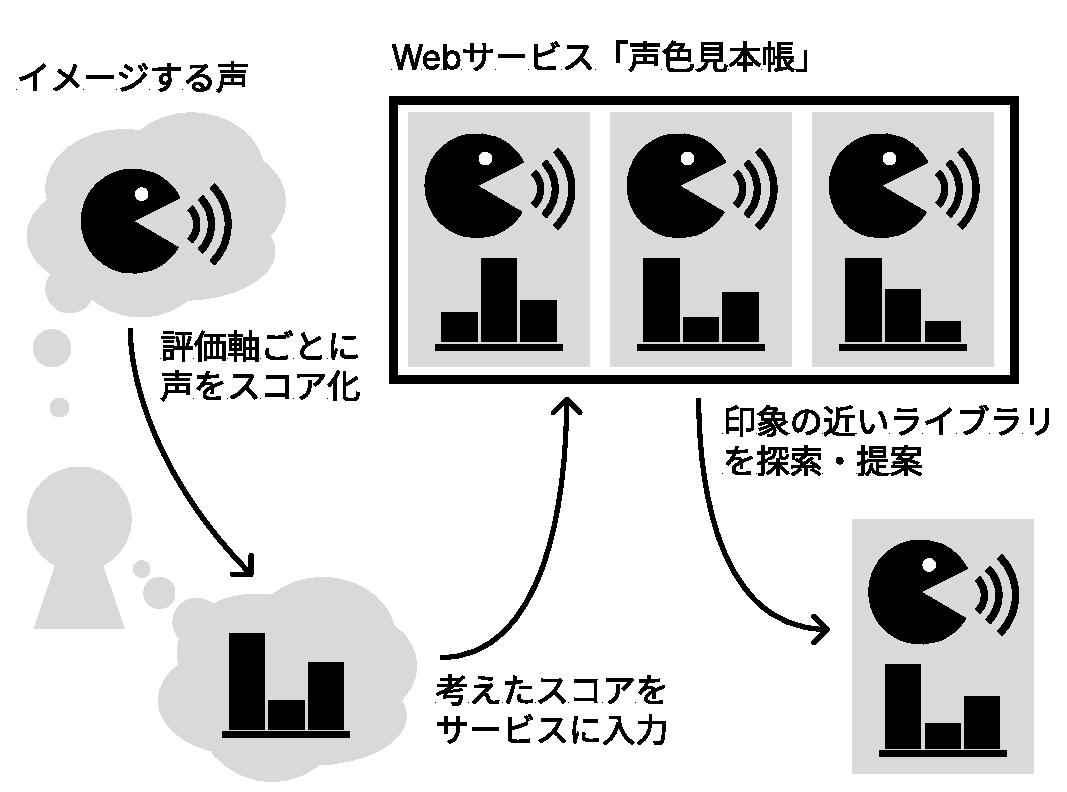
\includegraphics[width=0.9\linewidth]{fig/fig1.pdf}
  \caption{提案するサービス「声色見本帳」の概要}
  \label{fig:site_image}
\end{figure}

\begin{figure}[h]
  \centering
  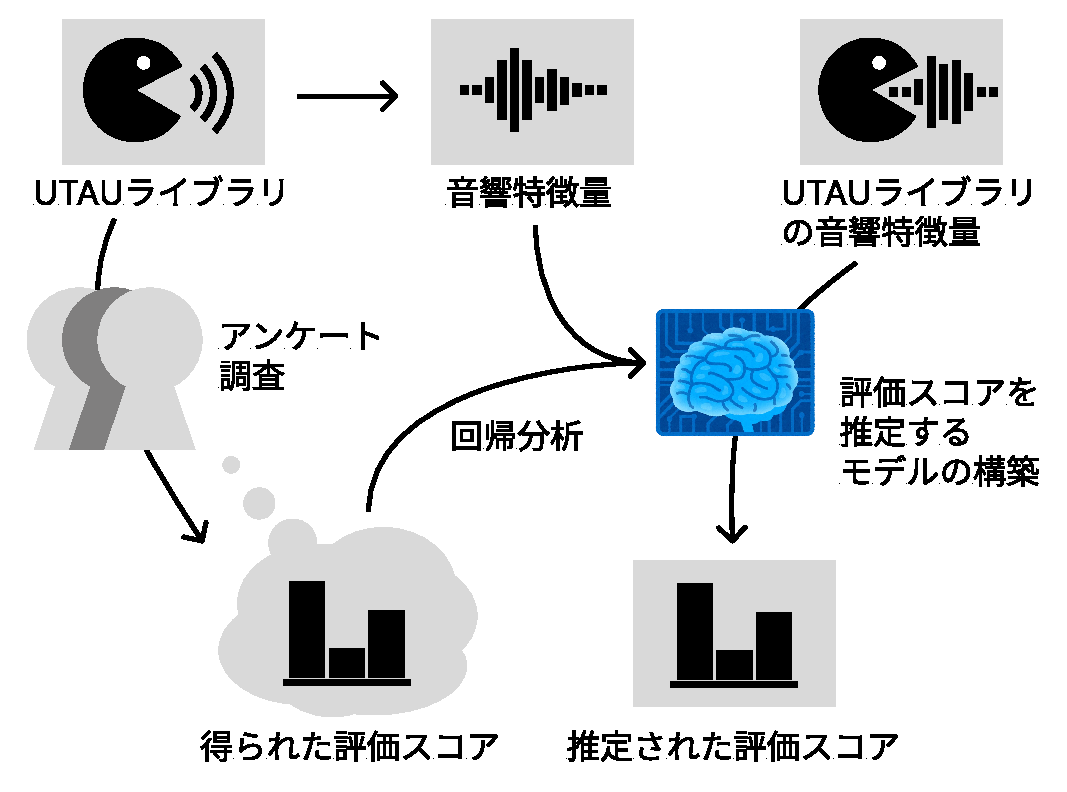
\includegraphics[width=0.9\linewidth]{fig/fig2.pdf}
  \caption{評価スコアを推定するモデルの構築イメージ}
  \label{fig:site_image}
\end{figure}

\section{本論文の構成}
本論文の構成は以下の通りである.
第2章では,関連研究について述べる.
第3章では,ライブラリから評価スコアを推定する機械学習モデルの構築と,構築したモデルの推論精度に対する評価実験について述べる.
第4章では,提案するサービス「声色見本帳」の設計と実装について述べる.
最後に第5章として本論文のまとめと今後の課題について述べる.

% Local Variables:
% mode: japanese-LaTeX
% TeX-master: "root"
% End:


\thispagestyle{myheadings}
\chapter{関連研究}
\label{sec:format}

\section{歌声に対して印象を推定する研究}
人の歌声を対象に,その印象を推定する研究は数多く存在する.
金礪らは歌唱の情報を可視化する手法を提案している\cite{impression}.
この研究では歌声から音響特徴量を抽出し,「迫力性」「丁寧さ」「明るさ」の3つの評価語に対するスコアを推定するモデルを作成している.
同著者による別の研究では,歌声の声質に対してイメージされる色を推定する試みも行っている\cite{voice_color}.

% 本研究に関連する研究として,人間の歌声の情報を理解しやすい形で可視化する研究\cite{impression, ama}がある.
% この研究では,ある程度の長さがある歌声と,そのうちの瞬間的な長さの歌声を用い,それぞれで印象を推定するモデルを作成している.
% ある程度の長さがある歌声では,迫力性,丁寧さ,明るさの3軸に対してそれぞれのスコアを推定するモデルを作成し,推定を行なった.
% 結果として,人の間でも印象の評価が大きく揺れるような歌唱などの例外を除き,十分な精度で印象を推定できた.
% また歌声のうち瞬間的な音声からは,印象に加えて声に対してイメージされる色を推定する試みも行っている.
% 彩度など色の要素と表現語の一つとして挙げられた活動性との関係が見られるなど,声質の色での表現に対して一定の有効性が示されたものの,他の要素との関係については今後の課題とされている.
% この研究から,声質へのなんらかの評価軸を用いた評価スコア付与が可能である点や,それを用いた声質の表現は一つの手段として妥当なものであると考えられる.

\section{合成音声の歌声にスコアを付与する研究}
UTAU音源を対象に声質に対し評価スコアを付与し,そのスコアを用いて音源を探索するシステムを提案する研究\cite{ong}が存在する.
この研究でも本研究と同じくUTAUに評価スコアを付与,探索システムを構築し,実際にユーザが求める声を探索できるかを確認している.
スコアの推定にはUTAUを用いて合成された音声データを用い,重回帰分析とカーネル回帰分析での推定制度の比較を行なっている.
また,推定されたスコアを用いて音源を探索する際には,ある2つのスコア行列間のユークリッド距離を目標類似距離とし,その逆数として定義した目標類似度を用いて音源を探索している.
評価実験では,ユーザのイメージする声に近いスコアを入力し,目標類似度の高いライブラリを提示した.するとユーザが求めるような声を持つライブラリを探索できる結果が示された.
一方でこの研究では,探索システムの実装に留まっており,探索アルゴリズムの検討や実際にユーザが利用できるサービスの提案は行われていない.

\section{可視化・探索するシステムを提供するサービス}
クリプトン・フューチャー・メディア株式会社と産業総合研究所によって開発された音楽発掘サービス「Kiite(キイテ)」では、その機能の一つとして「Kiite Radar」が提供されている\cite{kiite}.
ユーザは,楽曲の知名度やニコニコ動画上でのマイリスト率,楽曲を歌っているキャラクターなどの一般的な楽曲情報での絞り込みに限らず,楽曲の解析によって得られた曲の声質や踊りたくなるかどうかの印象をスライダーで設定し,その条件に合致する楽曲を探索するできる.
加えて,全ての楽曲を分析した印象に基づいて2次元平面上にプロットされた印象マップが提供されている.
激しい曲は左上に,軽快な曲は右上にプロットされるなど楽曲の配置には一定の傾向があり,ユーザはこれらを用いて直感的に楽曲を探索できる.
対象が歌声でなく楽曲である点は異なるが,本来数値ではない印象を数値化し,それを用いて可視化・探索するという点で本研究と共通する部分があり,サービスを提供する上で参考にできる.

% Local Variables:
% mode: japanese-LaTeX
% TeX-master: "root"
% End:


% \chapter{評価スコアを推定するモデルの構築}
\thispagestyle{myheadings}
\label{chap:model}

本章では,UTAU音源ライブラリに対して声質に対する評価スコアを付与するための機械学習モデルの概要と実装について述べる.
\ref{sec:utau}節では推論に用いるUTAU音源ライブラリとUTAU音源声質アンケートについて述べる.
\ref{sec:feature}節では使用する音声ファイルと音響特徴量,その抽出方法について述べる.
\ref{sec:model}節では評価スコアを推論する機械学習モデルの構築について述べ,\ref{sec:eval}節で構築したモデルの精度を評価する.

\section{UTAU音源ライブラリとUTAU音源声質アンケート}
\label{sec:utau}

本研究において探索対象とするUTAU音源ライブラリと,声質評価の基準として用いるUTAU音源声質アンケートについて説明する.
UTAU音源ライブラリは個人が作成・公開が可能で,ソフトと同じく無償で公開されているものが多い.
現在広く用いられている連続音方式であれば「あんああいあうあ」\cite{tatsu3shiki}といった形で複数の音素をできる限り一定の音程と音量になるように収録された肉声がwavファイルとして保存されいる.
UTAUは波形接続と呼ばれる手法を用いており,この音声データを切り貼りして歌声を合成し出力する.

UTAU音源声質アンケートはニコニコ大百科上で提言されたUTAU音源ライブラリに対してその声の特徴を評価するためのアンケート規格であり\cite{utausurvey},現在までにこの規格を用いて250種以上のUTAU音源ライブラリに対してアンケートが行われている.
このアンケートは表\ref{tab:survey}に示す7項目について,それぞれ1から7までの7段階評価で10件以上のアンケート調査を行い,その平均を評価値としている.

\begin{table}[htb]
  \centering
  \caption{UTAU音源声質アンケートの評価軸}
  \label{tab:survey}
  \begin{tabular}{c|cc}
    \hline
    評価軸 & 低い値の示す表現語 & 高い値の示す表現語 \\
    \hline
    声の性別 & 女性的 & 男性的 \\
    滑舌 & 舌足らず & はきはき \\
    特有性 & 素直 & 癖がある \\
    声の年齢 & 幼い & 大人びた \\
    透明感 & ノイジー & クリア \\
    声の強さ & 優しい & 力強い \\
    声の明度 & 暗い & 明るい \\
    \hline
  \end{tabular}
\end{table}

\section{特徴量の抽出}
\label{sec:feature}

UTAU音源ライブラリから推論に用いる音響特徴量を抽出する方法について述べる.
特徴量の抽出には,UTAU音源ライブラリから複数の音階で「あ」「い」「う」「え」「お」「ん」と発声した音声をライブラリ中の音声ファイルを直接操作して作成し,利用する.
五母音と子音「ん」は連続して発声のできる音素であり,安定して音声の特徴を抽出できる.
音声ファイルの操作時には,この範囲はUTAU上で音声が合成される際母音を伸ばすために用いる範囲である,子音部とブランクとしてライブラリに指定されるタイミング間の音声を利用した.
図\ref{fig:waveform}に「あ」を発生している音声ファイルの波形とスペクトログラム,ライブラリに指定されるタイミングの例を示す.
この図はUTAU互換ソフトウェアであるOpenUTAUからキャプチャしたものである.
波形上に塗られた赤いエリアの終わりが子音部,右端の青色の縦線がブランクとして指定されたタイミングを示す.
この範囲は音声の発声始めや次の音素の発音に移る部分を含まないため,音声波形とスペクトログラムの形状が安定している.
安定した声が収録されているため音声の特徴を抽出する上で適していると考えた.
音階はA3,D4,G4,C5,F5の5音階を用いる.
複数の音階を用いる特徴量の数を増加させるほか,音声の音域による特徴への影響などを反映できると考えられる.
複数音階の音声の生成には,ライブラリで音階ごとに指定される適切な音声ファイルからピッチシフトを行い生成した.

\begin{figure}[htb]
  \centering
  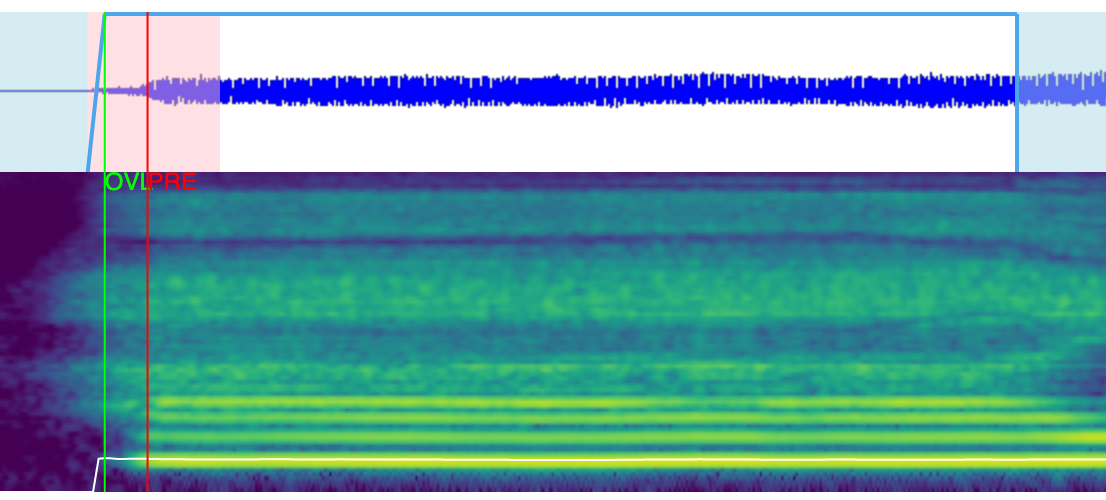
\includegraphics[width=0.9\linewidth]{fig/eve_a.png}
  \caption{音声ファイルの波形とスペクトログラム,ライブラリに指定されるタイミング}
  \label{fig:waveform}
\end{figure}

実際に用いる特徴量としては,MFCC,ZCR,F1〜F4の周波数を採用した.
Pythonライブラリであるlibrosaを用いて各音階と音素ごとにこれらの特徴量を抽出し,評価スコアの推論に用いた.
以下にそれぞれの特徴量について説明する.

MFCCはメル周波数ケプストラム係数の略で,音声の周波数成分を人間の聴覚特性に基づいて変換した数列である.
音声信号に対してフーリエ変換を適用して得られる周波数スペクトルを,人間の聴覚特性に合わせて変換(メルスケール変換)し,さらに対数変換と離散コサイン変換を適用して得られる.
周波数スペクトルと比較してMFCCは聴覚特性に合わせた特徴量を持つため,人間からの聞こえ方の特徴をよく反映しており,小島らによる歌声の印象評価と音響特徴量の関係についての研究\cite{mfcc_cute}ではMFCCが歌声の声質評価に有用だと示されている.
本研究では生成した音声からMFCCを64次元まで取得し用いる.

ZCRは音声の波形が0を交差する頻度を表す指標であり,音声信号の時間軸上で波形が正から負,または負から正に変化する回数を示す.
高い音声ほど周波数が高くなり波形の変化が多くなるためZCRも高くなるほか,摩擦音のような雑音成分が多い音声でもZCRは高くなる.
音声の声高を固定した今回の音声であれば,音声の透明感などに関連する指標として扱えると考え採用した.

フォルマントは周波数スペクトルのピークの周波数であり,周波数の低いものから順にF1,F2,と言った具合に呼ばれる.
フォルマントは声質や音素の音色に大きく関係する特徴量で特に母音の認識に重要とされており,音声の母音によってそのフォルマント周波数には一定の傾向がある.
粕谷らの研究によれば,同じ母音のフォルマント周波数でも話者の年齢や性別によって変化があり\cite{formant},声の性別感や年齢感に影響があると考えられる.

\section{モデルの構築}
\label{sec:model}

モデルの構築にはPythonライブラリであるPyCaretを用いた.
PyCaretは機械学習モデルの作成を簡略化するためのライブラリであり,データの前処理からモデルの選定,評価までを一連の流れで行える.
各評価スコアを推論の目標として与え,先述の特徴量から評価スコアを推定するモデルを評価スコアの7軸それぞれについて別々に作成した.

UTAU音源声質アンケートの結果はExcelファイルとして提供されている.
このファイルに記載されている240種のUTAU音源ライブラリのうち,現在でもダウンロードが可能であり,必要な音素が収録されていて,かつ利用規約上で研究目的を含む機械学習用途での利用が禁止されていない168ライブラリを学習対象とした.
データセットは学習データとテストデータに分割し,ランダムに選択した30\%をテストデータ,残りの70\%を学習データとして使用した.

7つの評価軸それぞれについてPyCaretで選択できるモデルごとの推定精度を比較した結果,全体的に精度の優れていたAdaBoost Regressorを選択した.
学習モデルを選択する際は,ランダムフォレストなどの離散モデルではなく線形回帰などの連続モデルの中から選択した.
これは連続量である特徴量から連続量である評価スコアを推定するため一定の値のみを推定結果に取る離散モデルよりも適していると考えたほか,予備実験において離散モデルでの学習時に過学習の傾向が頻繁に見られたためである.

\section{結果の評価}
\label{sec:eval}

構築したモデルによる推論の精度を評価するため,テストデータに対して推論を行い得た値と実際のアンケートによって得られた値を比較する.
テストデータは先述の通り学習データから各評価軸ごとにランダムに選ばれたデータであり,対象とした168ライブラリの3割にあたる51ライブラリを用いた.

図\ref{tab:score_box}では,横軸は評価軸を,縦軸はテストデータにおける実際の値と推測された値との誤差の二乗平均平方根(Root Mean Square Error: RMSE),エラーバーは誤差の標準偏差を示している.
RMSEは実際の値と推測された値の差を二乗して平均を取った後に平方根を求めたもので,数値予測モデルの精度を評価する際によく用いられる指標である.
結果を見ると,RMSEの最も小さい「滑舌」の軸では0.72,最も大きい「声の性別」の軸では1.27を示しており,評価軸ごとに大きな差は見られなかった.
RMSEは0に近いほど予測精度の高さを示し,評価スコアが1から7の数値を取る点を考慮すると,全体的に中程度の精度が得られたと言える.
これらの結果は先行研究\cite{dnn}での報告値と近い値であり,音響特徴量を用いた機械学習モデルとして一定の妥当性を示した.
また,エラーバーの大きさから,評価軸ごとでの予測の安定性の差も確認できる.

\begin{figure}[htb]
  \centering
  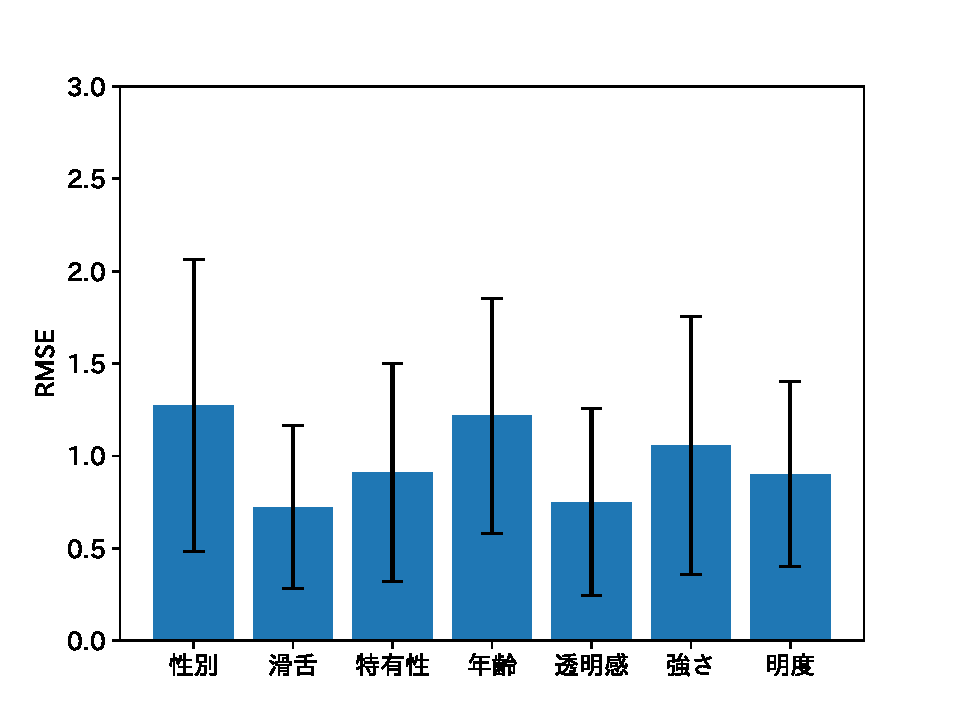
\includegraphics[width=\linewidth]{fig/rmse.pdf}
  \caption{テストデータとの誤差の二乗平均平方根}
  \label{tab:score_box}
\end{figure}

図\ref{tab:score_coor}では,横軸は評価軸を,縦軸はテストデータにおける実際の値と推測された値との相関係数を示している.
相関係数は一般に0.7以上であればデータ間に強い相関が,0.4以上であればある程度の相関があるとされ,実際の値と推測された値における相関が強いほど推論の精度が高いと言える.
結果を見ると,最も低い「声の年齢」は0.20とかなり低いものの,他の評価軸では0.49から0.66程度,最も高い「声の強さ」では0.66と,ある程度の相関が見られた.

\begin{figure}[htb]
  \centering
  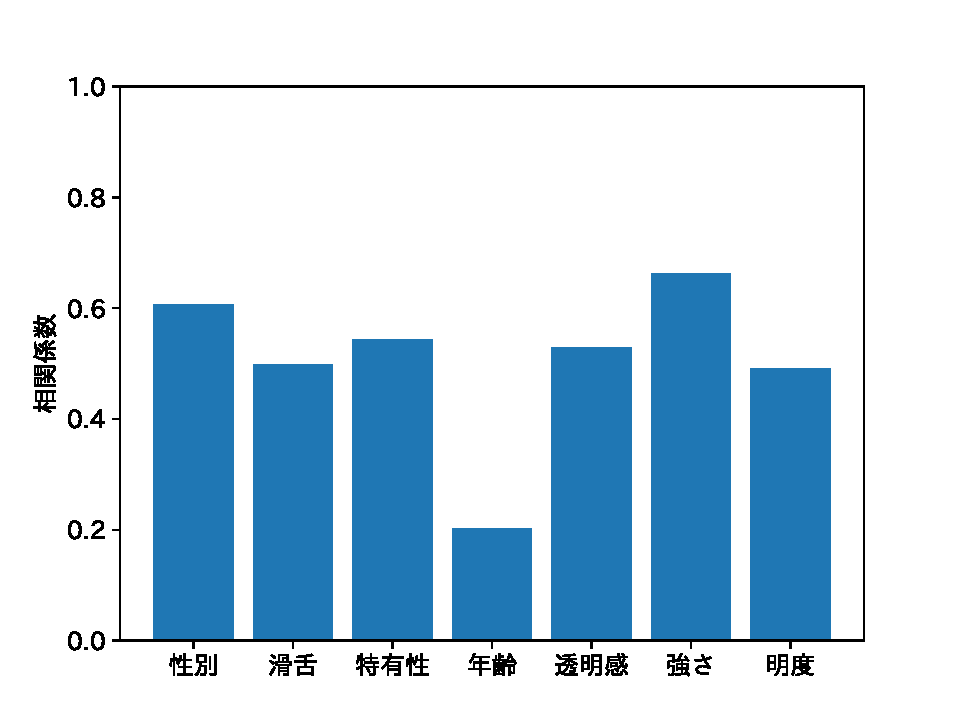
\includegraphics[width=\linewidth]{fig/coorpdf.pdf}
  \caption{テストデータとの相関係数}
  \label{tab:score_coor}
\end{figure}

7つの評価軸ごとの予測された値と実際の値との散布図を図\ref{fig:scatters}に示す.
図を見ると,相関係数の高かった「声の強さ」は右肩上がりの傾向が見られ相関の存在が分かる一方で,最も低かった「声の年齢」では点が縦に長く分布しているのが分かる.
これは相関の弱さだけでなく,実際の値はスコア範囲中に広く分布しているにも関わらず,予測された値がおおよそ3〜5と範囲の中央に偏っている現状を示している.
このような傾向は程度の差はあるものの他の評価軸でも見られ,精度を下げてる一因となっている.

\begin{figure}[htb]
  \centering
  \subcaptionbox{声の性別}{
  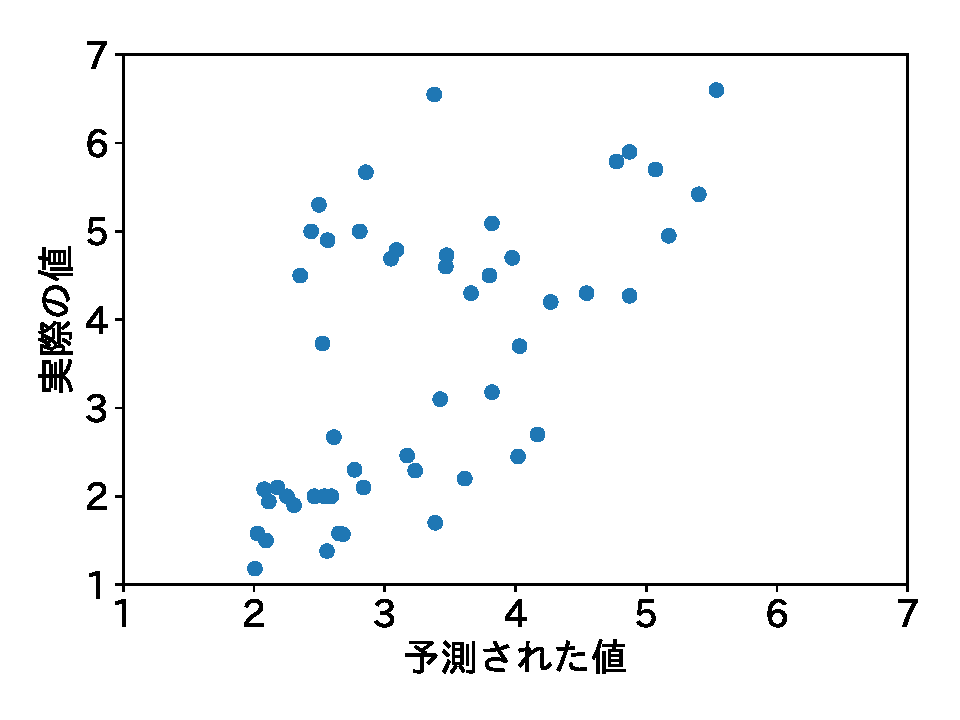
\includegraphics[width=0.4\linewidth]{fig/scatter/0.pdf}}
  \hspace{3mm}
  \subcaptionbox{滑舌}{
  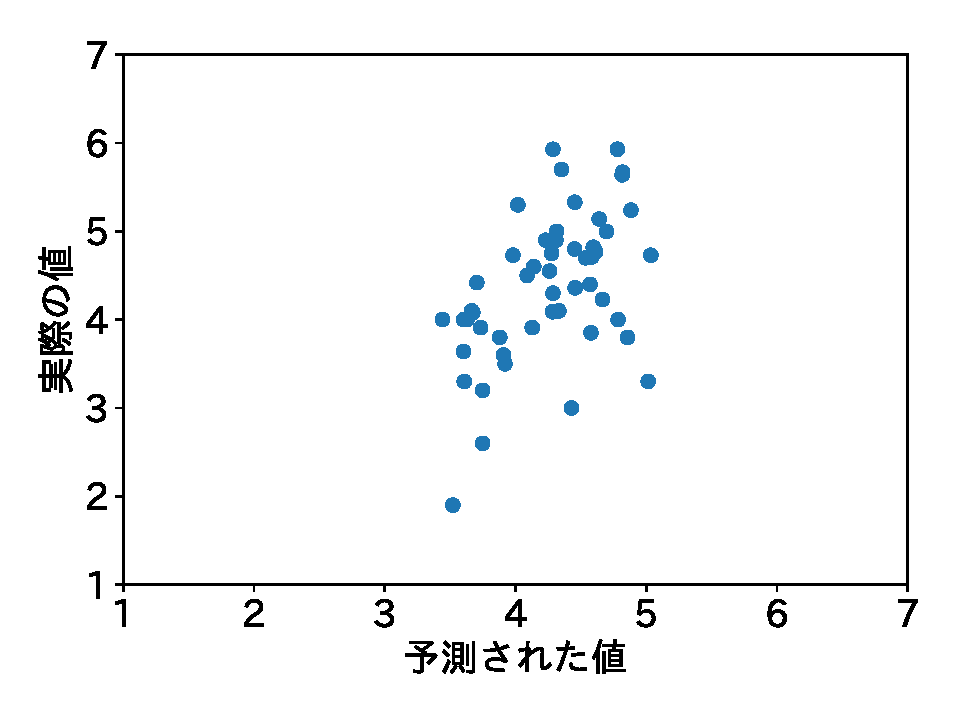
\includegraphics[width=0.4\linewidth]{fig/scatter/1.pdf}}
  \vspace{3mm}
  \subcaptionbox{特有性}{
  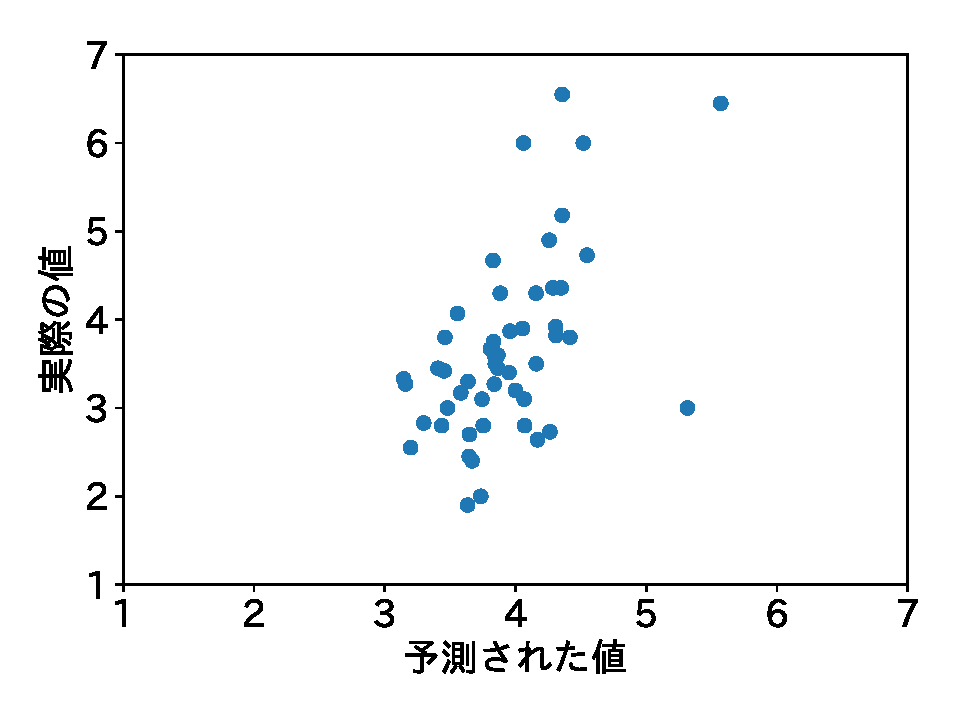
\includegraphics[width=0.4\linewidth]{fig/scatter/2.pdf}}
  \hspace{3mm}
  \subcaptionbox{声の年齢}{
  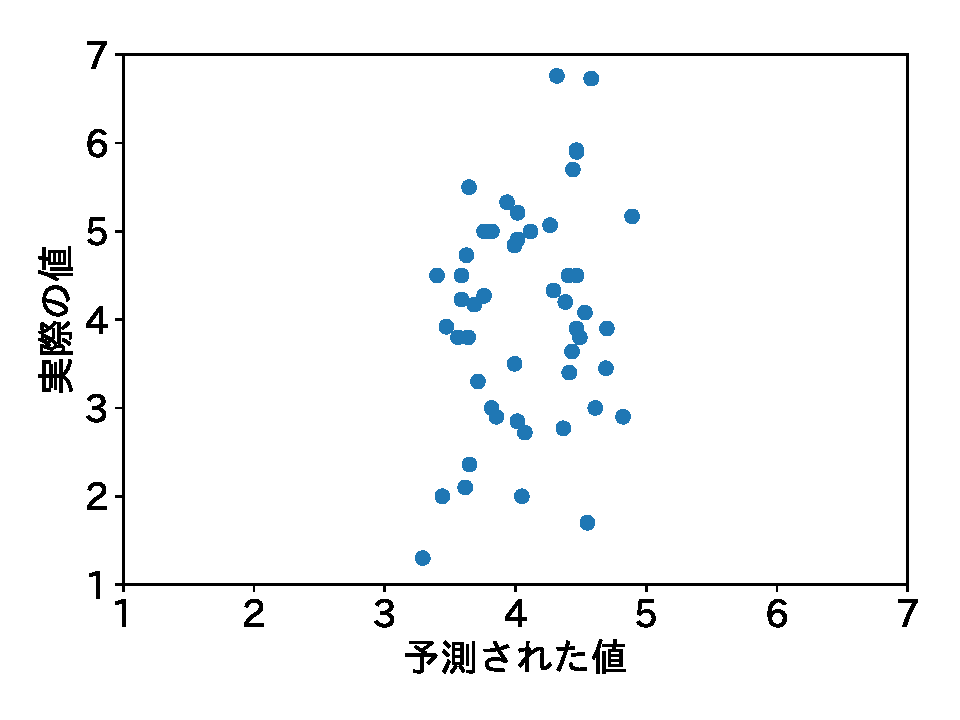
\includegraphics[width=0.4\linewidth]{fig/scatter/3.pdf}}
  \vspace{3mm}
  \subcaptionbox{透明感}{
  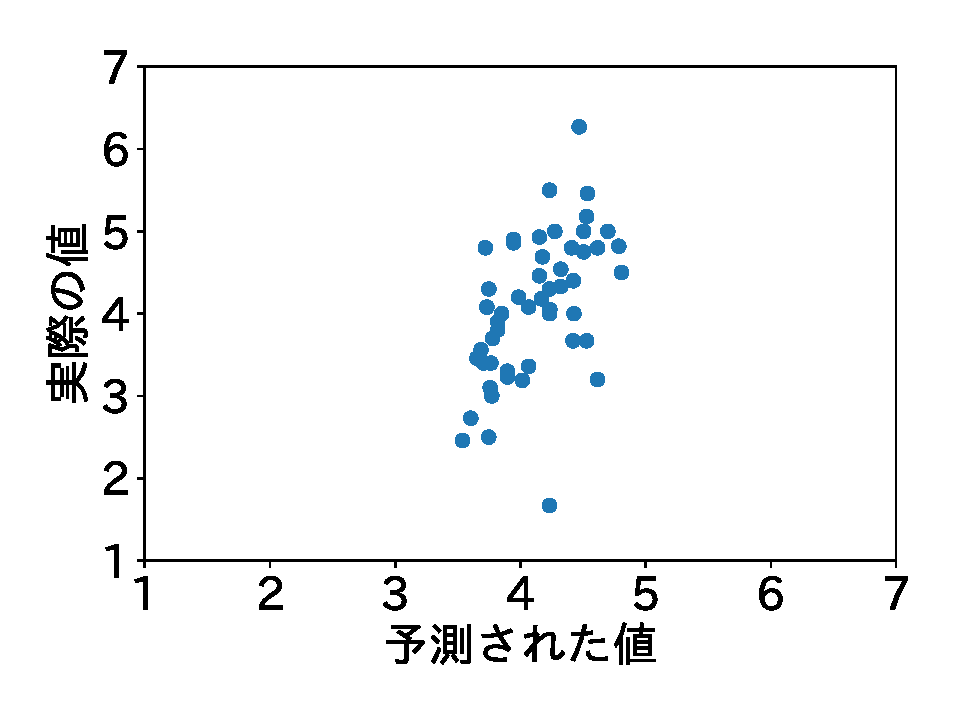
\includegraphics[width=0.4\linewidth]{fig/scatter/4.pdf}}
  \hspace{3mm}
  \subcaptionbox{声の強さ}{
  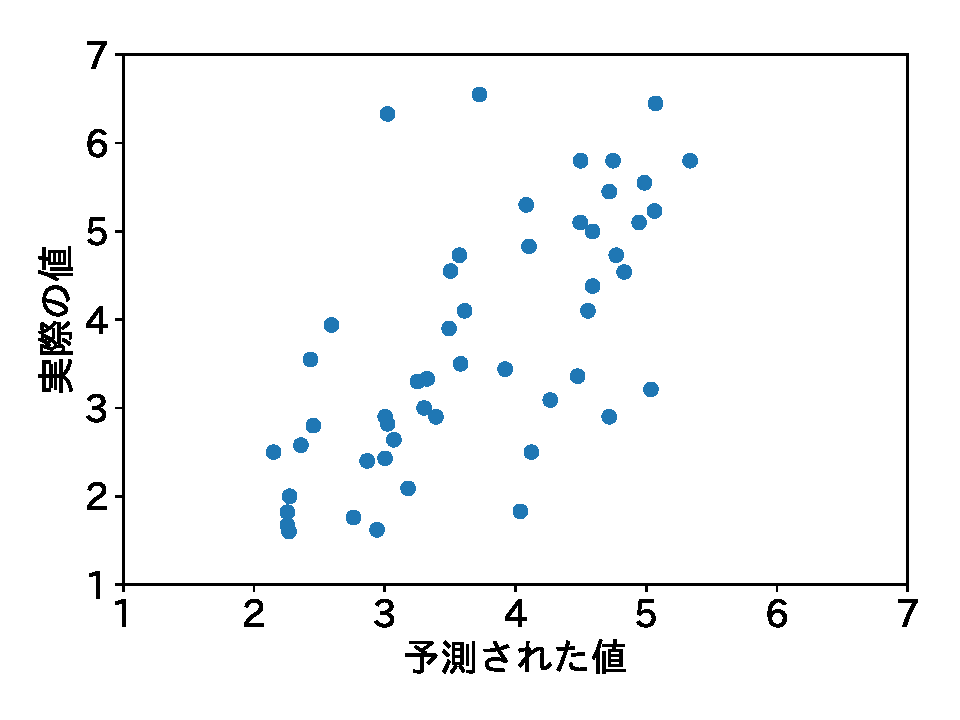
\includegraphics[width=0.4\linewidth]{fig/scatter/5.pdf}}
  \vspace{3mm}
  \subcaptionbox{声の明度}{
  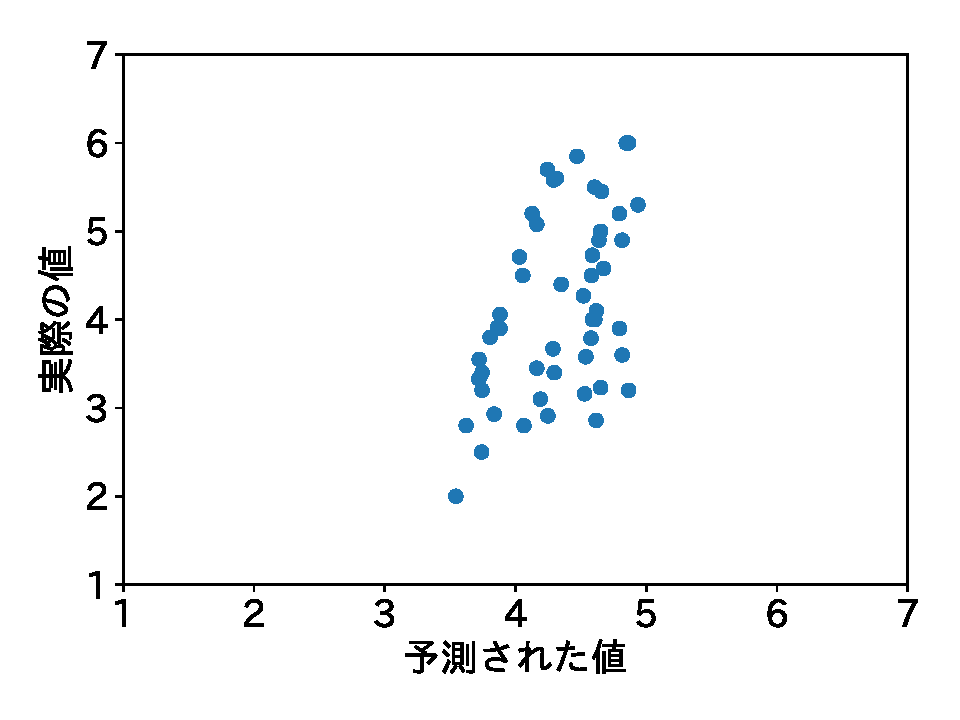
\includegraphics[width=0.4\linewidth]{fig/scatter/6.pdf}}
  \caption{実際の値と推測された値の散布図}
  \label{fig:scatters}
\end{figure}

予測値が中央に偏る現象について,一般にはデータの偏りやモデルの過学習,特徴量の不足などが要因とされている.
学習データを確認したが,テストデータのスコア分布からも分かるように,実際のスコアは広く分布しておりスコアの偏りは認められなかったほか,モデルの過学習についてもそのような傾向は見られなかった.
一方で,今回用いた音声特徴量が声質の印象に対し十分でなかった可能性は十分に考えられる.
主に母音に対して音階ごとに別々の特徴量を抽出したが,本研究で用いなかった子音にまつわる特徴量や音素間の遷移の特徴などの特徴量も声の印象に影響していると考えられる.
そのほか先行研究\cite{dnn}では機械学習の手法としてディープラーニングのモデルが採用されていたように,学習手法も複数のものが考えられる.
様々な手法を試し,より適したものに変更すれば性能向上の余地があると考えられる.

% Local Variables:
% mode: japanese-LaTeX
% TeX-master: "root"
% End:


% \chapter{声色見本帳}
\thispagestyle{myheadings}

本研究で提案するサービス「声色見本帳」は,ユーザが求める声の評価スコアを入力し,その評価スコアに近い合成音声ライブラリを探索・提案するサービスである.
ユーザは自身が求める声に近いライブラリを,多くのライブラリの声を手探りで聞き比べる手間なく自身に合った声を探索できる.
ライブラリの作成者も,自身のライブラリを多くのユーザに知ってもらう機会を得られる.
実際に作成したサービスの画面を図\ref{fig:site_image}に示す.

\begin{figure}[h]
  \centering
  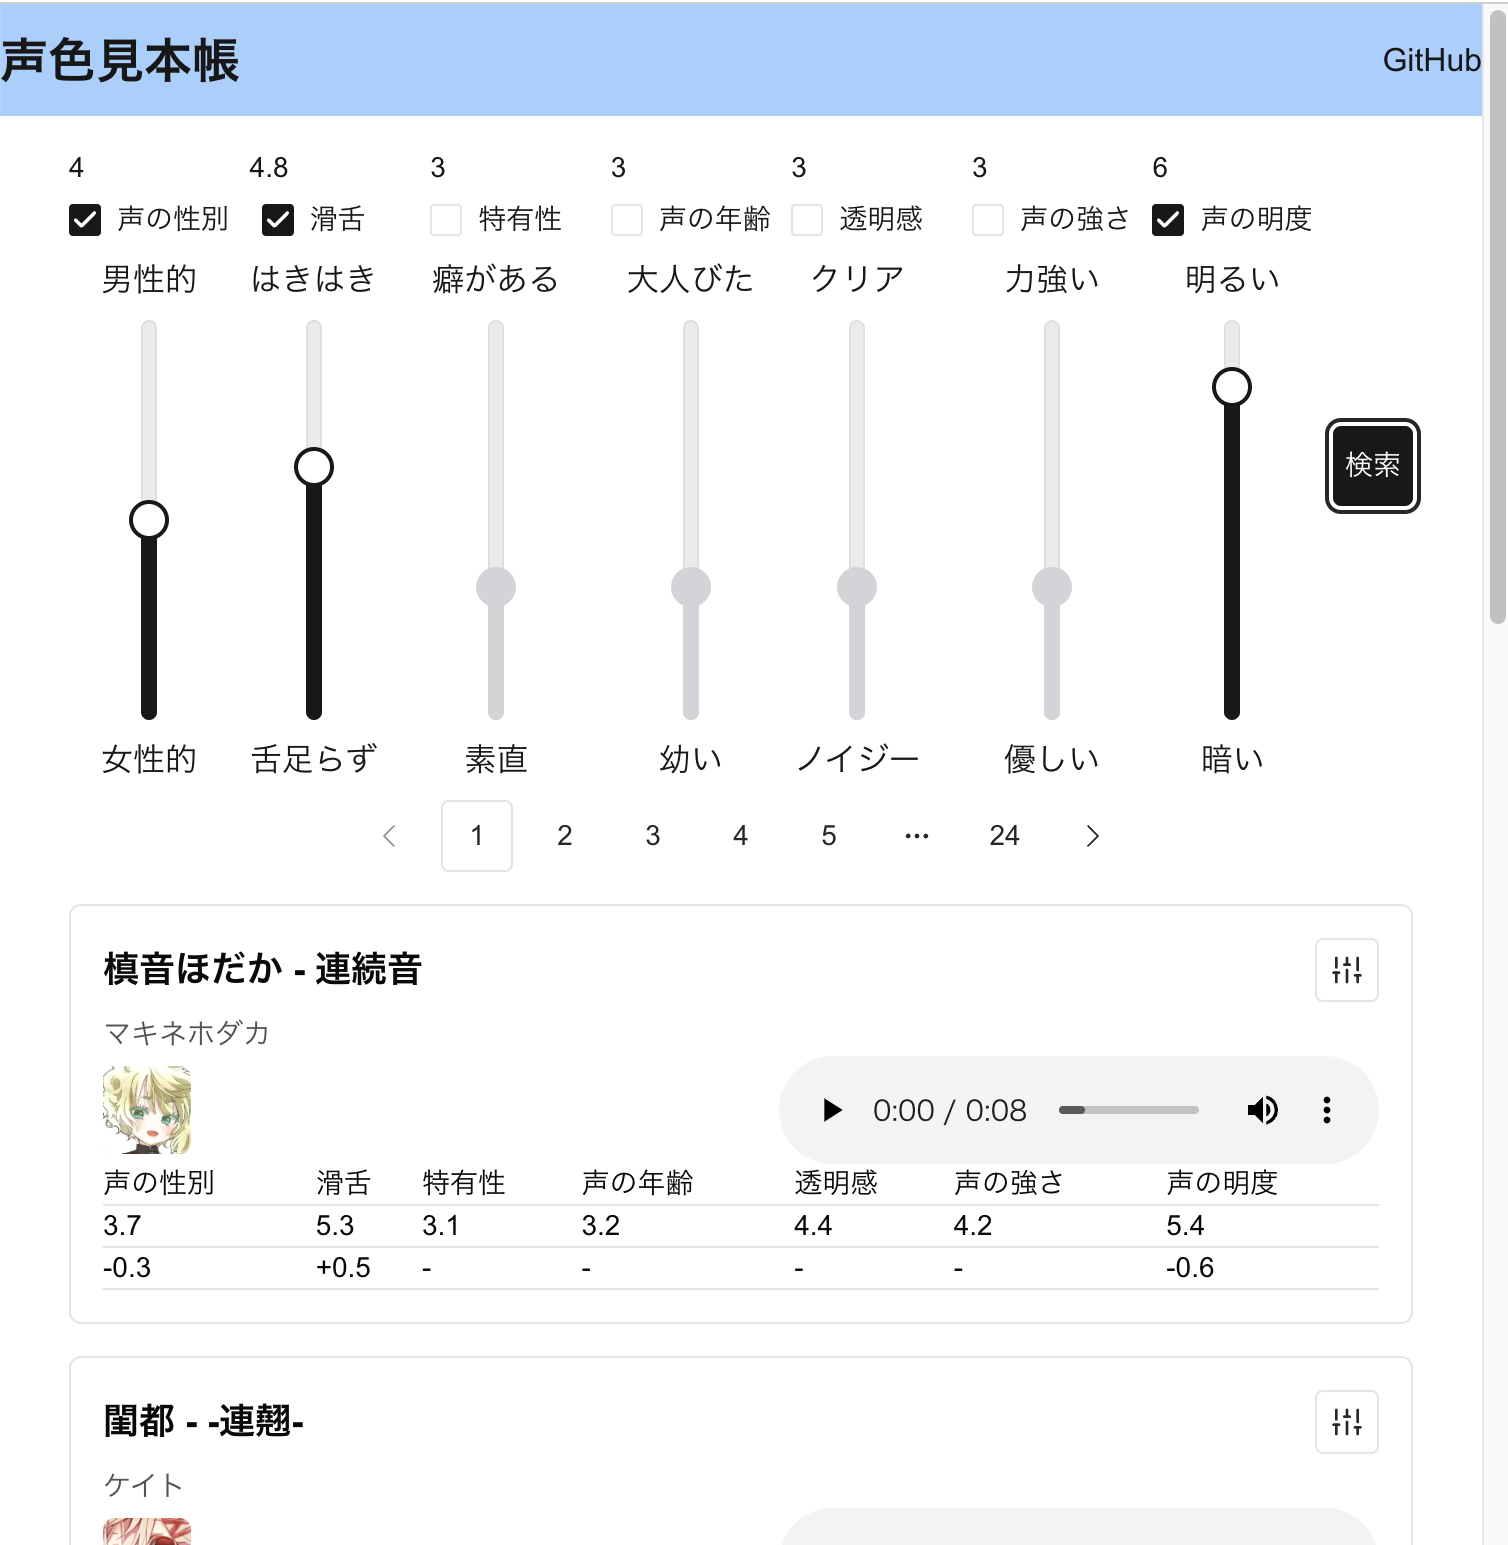
\includegraphics[width=0.9\linewidth]{fig/site_image.png}
  \caption{サービスの画面イメージ}
  \label{fig:site_image}
\end{figure}

\section{要求仕様}

本研究で提案するサービスについての要求仕様を以下に示す.
ユーザは求める声の評価スコアを数値として入力し,その評価スコアに近いUTAU音源ライブラリを探索できる.
探索結果として提示されたライブラリの歌声を実際に聞ける機能も必要である.
評価スコアを用いて声質を表現できるとしても,実際に聞いてみて本当に入力した評価スコアが求める声に近いかを確認したり,探索結果として提示されたライブラリの中から好みの声を選べる.
探索結果からは配布ページへのリンクを確認でき,ユーザがスムーズにライブラリをダウンロードできる.
また,ユーザが新しいライブラリを追加できる機能も提供する.
追加されたライブラリはサービスに登録されると同時に評価スコアが自動で推定され,以降の探索対象として利用される.
この機能により,サービスに登録されていなかったライブラリや,今後公開されるライブラリも将来的に探索できる.
サービスはWebサービスとして実装し,ユーザがブラウザから手軽に利用できるかたちにする.
合成音声ソフトウェアであるUTAUはスマートフォンではなくPCでの利用が一般的であるため,そのライブラリの探索もPCで行うのが自然である.
よってサービスはPCでの利用を前提としてデザインを行う.

\section{実装}
サービスのフロントエンドはTypeScriptを用いて開発し,フレームワークとしてNext.js,UIコンポーネントライブラリとしてChakra UIを用いて実装した.
バックエンドはPythonを用いて開発し,フレームワークとしてFastAPIを,データベースとしてはPostgreSQLを用いて実装した.
バックエンドをPythonで実装したため,ライブラリを追加する際事前に構築した機械学習モデルによる推論やサンプル音声の合成を一挙に行える.

\subsection{ライブラリ探索機能}

探索はサービスのトップ画面から行う.
ユーザは求める声の評価スコアを7つの評価軸に対してスライダーを用いて評価スコアを0.1刻みの小数で入力した後,探索ボタンをクリックして探索を行う.
スライダーによる入力インタフェースに加えそのスライダーの両端に評価スコアの高低に対応する表現語を配置したため,数値である評価スコアと表現語の表す声との関係を直感的に理解できる.
探索ボタンをクリックするとAPIを通じてデータベースにアクセスし,入力された評価スコアに近いライブラリを探索し,その結果をユーザに提示する.

入力の際,ユーザは各評価軸ごとに存在するチェックボックスを操作できる.
チェックボックスはデフォルトでは全てチェックされており,チェックを外すと対応する評価軸を無効化できる.
無効化された評価軸はスライダーもグレーアウト状態になり操作できなくなり,探索時にその評価軸が無視される.
この機能は,ユーザにとって7つの評価軸全てに対する求めたい声の評価スコアの想定と入力は煩雑であると考え実装した.
この機能によってユーザは自身の重視するいくつかの評価軸に対してのみ評価スコアを入力し,他の評価軸については入力せずに探索できる.

評価スコアが近いかの評価には,ユーザに選択された評価軸での平方ユークリッド距離を用いる.
ライブラリに対して推定された評価スコアと,ユーザが入力した評価スコアとの差分を各評価軸ごとに計算した後,その差分の二乗和を計算して評価スコア間の距離を求める.
この際,チェックボックスで無効化された評価軸については差分の計算を行わず,評価スコアの距離に影響を与えないようにする.
距離が小さい順にライブラリを並び替え,探索結果として表示する.
この方法は探索のたびに全てのライブラリに対して距離の計算を行うため,ライブラリの増加に伴い計算量が増加してしまうが,ライブラリの数が数百程度であれば十分な速度で探索が行えたため,現状の規模では問題ないと判断した.
今後登録ライブラリ数が増加し探索速度に大きな影響が見られた場合は探索の高速化を検討する必要がある.
探索の高速化の方法としては,探索結果をキャッシュして再探索時の高速化を図る方法や,ライブラリをその評価値によって事前にクラスタリングし,クラスタごとに探索を行う方法などが考えられる.

また,探索結果として表示されたライブラリを選択し,その評価スコアを入力欄に転写できる機能を実装した.
あるライブラリの評価スコアを探索にそのまま用いると,そのライブラリに近い声質のライブラリを探せる.

\subsection{ライブラリ情報の表示}

探索結果として,各ライブラリの名前やアイコン,推定された評価スコアなどライブラリの情報を表示する.
評価スコアは評価軸ごとに探索に用いたスコアとの差分も表示し,求める声とどのような違いがあるかを一目でわかるようにした.
ライブラリのスコア表示は探索時に入力したスライダーと同じ向きに同じ並びで表示されるため,余計なストレスなくスコアを比較できる.

ライブラリの声について実際に聞いて比較できるよう,ライブラリ情報の中にライブラリの歌声を再生できるメディアプレーヤを設置した.
歌声の確認に用いるサンプル音声として事前に楽曲の一部を歌わせた音声ファイルを用いた.
歌わせる楽曲としては童謡の「かえるのうた」を選定し,最初の一節を対象とした.

本サービスはユーザが求める声に近いライブラリを探索するサービスだが,探索した後にライブラリをダウンロードする機能までは提供しない.
これはダウンロード時にライブラリのライセンスや利用規約を確認する必要があるが,その確認をサービス内で行うのが難しいためである.
そのため,ライブラリ情報からライブラリの配布ページへ遷移できるリンクを設置した.
ユーザはこのリンクからライブラリの配布ページにアクセスし,先方で示されるライセンスや利用規約を確認した上でダウンロードを行える.

\subsection{探索対象ライブラリの追加}

ユーザはライブラリ追加画面から未登録のライブラリを検索対象として登録できる.
追加する際はライブラリの名前やバージョン,配布ページのURLなどの情報を入力し,UTAU音源ファイルをzipファイルとアップロードする.
バックエンドではアップロードされたzipファイルを展開し,\ref{chap:model}章で述べたように音響特徴量を抽出し,構築済みの機械学習モデルで評価スコアを推定する.
アップロードされたファイルは各種データの生成後には必要がなくなるが,今後推論モデルを変更したり,再度サンプル音声を生成する必要が生まれる場合を想定し,zipファイルの状態で保存しておく.

アップロード時には合わせてサンプル音声の合成も行う.
一般的にUTAU音源ライブラリを扱うソフトウェアであるUTAUやOpenUTAUはCLI上での動作に対応しておらず,自動的な処理に対応していない.
そこでサンプル音声の合成には,Pythonによる音楽・歌声シンセサイザインタフェースであるScoreDraftを用いて合成を行った.
このライブラリはPythonからUTAU音源ライブラリを用いた音声合成が行えるため,サーバ上での自動的な処理に適している.

これらの処理が完了すると,ライブラリの情報と推定された評価スコア,合成されたサンプル音声がデータベースに登録され,以降の探索で利用できるようになる.
アップロードされたファイルから評価スコアの推定やサンプル音声の合成を含む一連の処理は大きく時間はかからないが,UTAU音源ファイルのアップロードには数十秒ほどかかるため,ユーザにアップロード進捗を伝えるためアップロード完了までプログレスバーを表示する.
アップロード完了画面では,上記のプログレスバーと,処理の完了後には推定されたスコアなどを表示する.

% Local Variables:
% mode: japanese-LaTeX
% TeX-master: "root"
% End:


% \chapter{おわりに}
\thispagestyle{myheadings}

\section{まとめ}
本研究では合成音声ライブラリが多く存在する中で,ユーザが用途に合った声を探索するための手法として,声の印象を数値化し,それを用いてライブラリを探索するWebサービス「声色見本帳」を提案した.
まず,UTAU音源の声から声の印象を数値化する機械学習モデルを構築した.
モデルは入力データとして音声から抽出したMFCCをはじめとする音響特徴量を,出力データとして声の印象を7つの評価軸ごとに数値化した評価スコアを取る.
入力データはPythonライブラリであるlibrosaを用いて抽出し,学習時に用いる評価スコアには既存のUTAU音源声質アンケートの結果を用いた.
モデル構築にはPythonライブラリであるPyCaretを用い,学習方法にはAdaBoost Regressorを,教師データとして声に対する既存のアンケート結果から168ライブラリ分のデータを用いた.
構築したモデルの推論精度を確認するため評価実験を行い,評価軸ごとの相関係数が概ね0.5〜0.6となる結果を得,一定の精度での推定を確認した.
一方で,「声の年齢」をはじめとする複数の評価軸では予測値が評価スコア範囲中央に偏るなどの問題が見られた.

ユーザが求める声の印象を評価スコアとして入力し,声の近いライブラリを探索できるWebサービス「声色見本帳」を実装した.
ライブラリ探索に用いるライブラリごとの評価スコアは,先立って構築した機械学習モデルを用いて事前に推定し付与する.
サービスはユーザの求める声に近いライブラリを複数提案し,それらのサンプル音声やダウンロードページへのリンクを提供する.
気軽に利用できるWebサービスを通じて目的に適した声との出会いを促進し,求める声質を持つライブラリを効率的に探索できたり,埋もれがちな多様なライブラリへ活用機会の増加が期待できる.

\section{今後の課題}
今後の課題としては,まず機械学習モデルの改善が挙げられる.
改善手法として,より多角的な音響特徴量の利用が考えられる.
本研究でモデルの入力として用いた音響特徴量は,主に母音の発声から特徴量を抽出している.
しかし,子音にまつわる特徴量や,子音を含む音素間の遷移にまつわる特徴量などから声の印象を得られると考えられる.
これらを用いてモデルの入力データの表現力を向上させれば,より適切に声の印象を推定できる.

また,運用されるサービスを活用し,学習データの拡充も考えられる.
例えば,ユーザの探索履歴を収集し,あるユーザの探索パラメータと実際にダウンロードページにアクセスした音源との関連付けを行い,学習データとしての利用が考えられる.
あるいはより直接的に,音源ごとにユーザから評価の投票を募り,その結果を用いるなど,ユーザからのフィードバックを利用した手法も考えられる.
学習データをより多様で正確なものにすれば,モデルの汎用性向上が期待できる.

サービスとしての利便性向上も課題である.
現在,ライブラリの新規追加時にはUTAU音源ファイルをzipファイルでアップロードする形式であるが,このファイルは数百MBのものも多く,アップロードに時間がかかる問題がある.
サービスの運用にはこの音源ファイルそのものは必要ないため,ユーザのローカル環境上で音声ファイルの解析とサンプル音声の生成が出来れば,その結果を送るのみで済むため通信時間の大幅な削減が期待できる.
探索システムの改善としては,現在評価スコアの類似度指標としてユークリッド距離を用いているが,それについて評価実験と検討が必要と感じている.
より本当にユークリッド距離は評価スコアの類似度を適切に表現できるのか,また他の指標を用いた場合の探索結果の変化について検討が必要である.
また,ライブラリ情報の更新・修正機能,あるいは権利者からの削除依頼への適切な対応体制の整備も必須である.これらの改善を行いより利便性の高いサービスを目指す.

% Local Variables:
% mode: japanese-LaTeX
% TeX-master: "root"
% End:


\chapter*{謝辞の例}
\addcontentsline{toc}{chapter}{\protect\numberline {} 謝辞の例}

本研究を進めるにあたり,多くの御指導,御鞭撻を賜わりました
愛知工大教授に深く感謝致します.

また,御討論、御助言していただきました,
○×大学工学部電子情報工学科の山谷川介教授,および山谷研究室のみなさん
に深く感謝致します.

最後に,日頃から熱心に討論,助言してくださいました
愛知研究室のみなさんに深く感謝致します.

% Local Variables: 
% mode: latex
% TeX-master: "root"
% End: 


\thispagestyle{myheadings}
\addcontentsline{toc}{chapter}{\protect\numberline {} 参考文献}

\begin{thebibliography}{参考文献}

\bibitem{mycoeiroink}
COEIROINC,
MYCOEIROINK.
\url{https://coeiroink.com/mycoeiroink/list}

\bibitem{vdbutau}
Vocaloid Database.
\url{https://vocadb.net/Search?searchType=Artist&artistType=UTAU}

\bibitem{pop}
金礪 愛,中野 倫靖,後藤 真孝,菊池 英明,
ポピュラー音楽における歌声の印象評価語を自動推定するシステム.
情報処理学会論文誌,Vol.2013-MUS-100,No.19,pp.1-8,2013

\bibitem{voice_color}
金礪 愛,菊池 英明,
歌唱音声における声質の特徴と想起される色の関係.
日本感性工学会論文誌,17巻,1号,pp.109-118,2018

\bibitem{impression}
金礪 愛,中野 倫靖,後藤 真孝,菊池 英明,
歌声の印象評価尺度の構築に基づく多様な印象の自動推定手法.
情報処理学会論文誌,Vol.57,No.5,pp.1375-1388,2016

\bibitem{ama}
金礪愛,
アマチュア歌唱者に向けた歌声可視化方法の検討.
博士論文,早稲田大学,2018

\bibitem{ong}
山根壮一ほか,
歌声合成システムの音源データに対する声質推定と声質制御.
情報処理学会研究報告,Vol.2015-MUS-108,No.6,pp.1-6,2015

\bibitem{dnn}
横森文哉,大柴まりや,森勢将雅,小澤賢司,
スペクトル包絡情報を入力としたDeep Neural Networkに基づく歌声のための声質評価
情報処理学会音楽情報科学研究会,Vol.2015-MUS-107,No.61,1-6,2015

\bibitem{zcr}
佐賀 圭真,井村 誠孝,
発話音声の聞き取りやすさ向上のための音声特徴量解析.
エンタテインメントコンピューティングシンポジウム2019論文集,2019,pp.84-86,2019

\bibitem{formant}
粕谷英樹ほか,
年令, 性別による日本語5母音のピッチ周波数とホルマント周波数の変化,
日本音響学会誌,24巻,6号,pp.355-364,1968

\bibitem{kiite}
産業総合研究所,
音楽印象分析・音楽推薦を駆使して楽曲と出会える音楽発掘サービス「Kiite」を公開
\url{https://www.aist.go.jp/aist_j/press_release/pr2019/pr20190830/pr20190830.html}

\bibitem{tatsu3shiki}
巽式 連続音の録音リスト配布 - 巽のブログ,
\url{https://tatsu3.hateblo.jp/entry/ar426004}

\bibitem{utausurvey}
ニコニコ大百科,
UTAU音源声質アンケートとは,
% \url{https://dic.nicovideo.jp/a/utau%E9%9F%B3%E6%BA%90%E5%A3%B0%E8%B3%AA%E3%82%A2%E3%83%B3%E3%82%B1%E3%83%BC%E3%83%88}
\url{https://dic.nicovideo.jp/a/utau音源声質アンケート}

\end{thebibliography}
% Local Variables:
% mode: japanese-LaTeX
% TeX-master: "root"
% End:


% これ以降,付録となる
\appendix

\chapter{論文表紙}
\thispagestyle{myheadings}

\vspace{-1.0cm}

\begin{center}

{\LARGE 愛知工業大学情報科学部情報科学科\\
コンピュータシステム専攻(メディア情報専攻)

\vspace{1.0cm}

令和2年度~卒業論文\\

\vspace{2.0cm}

{\Huge 
\baselineskip=15mm
\textbf{オブジェクト指向データに対する\\
グラマーモデルの適用\\}}

\vspace{7.0cm}

2020年2月\\

\vspace{1.0cm}

\begin{tabular}[h]{lll}
  研究者  & K00001 & 愛工太郎\\
         & K00011 & 八草花子\\
         & X00012 & 愛知環状\\
\end{tabular}

\vspace{1.0cm}

指導教員\ \ 情報一郎\ \ 教授}

\end{center}

% Local Variables: 
% mode: latex
% TeX-master: "root"
% End: 


\end{document}

%%% Local Variables: 
%%% mode: latex
%%% TeX-master: t
%%% End: 
